% ANU ENGN4200 - Individual Project Thesis 2020 Template
% Originally supplied by Wojciech Lipinksi
% Modified and updated by Chris Bodger - u5395595 

\documentclass[a4paper,11pt]{report}

% import packages
\usepackage{anuthesis}
\usepackage{ucs}
\usepackage{inputenc}
%\usepackage[utf8x]{inputenc}
\usepackage{amsmath}
\usepackage{amsfonts}
\usepackage{amssymb}
\usepackage{amsthm}
\usepackage[australian]{babel}
\usepackage{fontenc}
\usepackage{graphicx}

\usepackage{comment}
\usepackage{mathrsfs}
\usepackage{booktabs}
\usepackage{hyperref}
\usepackage{fancyhdr}
\usepackage{fancyvrb}
\usepackage{subfig}
\usepackage{appendix}
\usepackage[bw,numbered]{mcode}
\usepackage[nottoc,numbib]{tocbibind}
\usepackage[square,numbers,sort]{natbib}



%===============================================================================
%             Margins
%===============================================================================
\usepackage[top=20mm, bottom=20mm ,left=20mm, right=20mm]{geometry}

%===============================================================================
%     Setting page header format
%===============================================================================
\pagestyle{fancyplain}
\renewcommand{\sectionmark}[1]{\markright{\thesection\ #1}{}}
\renewcommand{\chaptermark}[1]{\markboth{\chaptername\ \thechapter\ #1}{}}
\fancyhf{}
\lhead{\fancyplain{}{\leftmark}}
\rhead{\fancyplain{}{\rightmark}}
\rfoot{\textbf{\thepage}}

\makeatletter
\def\listoffigures{
\@restonecolfalse\if@twocolumn\@restonecoltrue\onecolumn
 \fi\chapter*{List of Figures\@mkboth{List of Figures}{List of Figures}}
 \@starttoc{lof}\if@restonecol\twocolumn\fi
 }
\makeatother


%===============================================================================
%             Authorship              
% These parameters are used throughtout the template. 
% Set the details to suit your project
%===============================================================================
\def\THETITLE{ArduPilot Implementation of Optimal Control for Tilt Rotor UAV Landing}
\title{\THETITLE}
\def\THEAUTHOR{Lincoln Karavas}
\author{\THEAUTHOR}
\def\studentID{U7091679}
\def\supervisor{Mr. Mathew Hampsey}
\def\examiner{Prof. Robert Mahony}
\date{\today}

\begin{document}
  \setcounter{secnumdepth}{5}
  \setcounter{tocdepth}{7}
  \linespread{1.2}
  \selectfont
  \pagenumbering{roman}  % first use Roman numerals for page numbers
  
  %=============================================================================
  %         Title Page
  %=============================================================================
  \begin{titlepage}
    %\enlargethispage{2cm}
    \vspace*{\fill}
    \begin{center}

      \makeatletter
      \huge\textbf{\THETITLE} \\[1.5cm]
      \large A thesis submitted in part fulfilment of the degree of \\
      \large Bachelor of Engineering (Honours)\\ [1.5cm]
      \large\textbf{by \\ \THEAUTHOR\ \\ \studentID} \\[1.5cm]
      \normalsize\textbf{Supervisor: \supervisor} \\[0.1cm]
      \normalsize\textbf{Examiner: \examiner} \\[1.5cm]
      %\thismonth
      \makeatother
      
      \vspace*{\fill}
      
\includegraphics[width=70mm]{images/logo} \\[3cm]
      \vspace*{-1.5cm}
      \Large College of Engineering and Computer Science\\
      The Australian National University \\ [1.5cm]
      \normalsize\thismonth \\
    \end{center}
    \vspace*{\fill}
  \end{titlepage}

  % include statements effectively insert the contents of the named file.
  % They are not necessary, but are useful for organising your work.
  % They always start a new page.
  
  %=============================================================================
  %         Plagerism
  %=============================================================================
  % includes the contents of the file plagerism-statement.tex
  \begin{titlepage}
\vspace*{\fill}
\noindent
This thesis contains no material which has been accepted for the award of any other degree or diploma in any university. To the best of the author’s knowledge, it contains no material previously published or written by another person, except where due reference is made in the text.
\\
\\
\\
\\
\hspace*{\fill}\THEAUTHOR \\
\hspace*{\fill}\today
	\vspace*{\fill}
\begin{center}
	\copyright\THEAUTHOR
\end{center}

\end{titlepage}

  %=============================================================================
  %       Acknowledgements
  %=============================================================================
  % include the contents of the file thanks.tex
  \chapter*{Acknowledgements}
\addcontentsline{toc}{chapter}{Acknowledgements}

Thanks to my cat, Fluffy and my budgie, Rex.
  
  
  
  %=============================================================================
  %         Abstract
  %=============================================================================
  % include the contents of the file abstract.tex
  \chapter*{Abstract}
\addcontentsline{toc}{chapter}{Abstract}

\vspace*{2em}
The abstract should be brief (100--150 words) and directed to readers familiar with the broad area of the thesis subject. ``The abstract is of utmost importance for it is read by 10 to 500 times more people than hear or read the entire article. It should not be a mere recital of the subjects covered, replete with such expressions as ``is discussed'' and ``is described.'' It should be a condensation and concentration of the essential qualities of the paper.''

  %=============================================================================
  %      Contents Page
  %=============================================================================
  \selectfont
  \tableofcontents

  %=============================================================================
  %      List of Figures
  %=============================================================================
  \listoffigures % makes a list of figures
  \addcontentsline{toc}{chapter}{List of Figures}

  %=============================================================================
  %      List of Tables
  %=============================================================================
  \listoftables  % uncomment this if you have tables
  \addcontentsline{toc}{chapter}{List of Tables}

  %=============================================================================
  %      Abbreviations
  %=============================================================================
  \selectfont
  \chapter*{Nomenclature}
\addcontentsline{toc}{chapter}{Nomenclature}

\begin{tabular}{p{0.8cm}p{2.5cm}l}
&SOS		& Save Our Souls \\
\end{tabular}



  % Change settings for for Thesis body
  \pagenumbering{arabic} % switch to Arabic numerals for page numbers
  \setcounter{page}{1}  % set page number to 1

  %=============================================================================
  %      Thesis Body
  %=============================================================================
  % includes contents of all sections to be displayed in the thesis document. uncomment the extra chapters if necessary
  \chapter{Introduction}
\vspace{-1.4em}
The introduction orients the reader to your thesis. It should present the nature and scope of the problem in terms of applications to `real world' problems (what motivates the study); refer briefly to associated and relevant literature already published; state the method of investigation (the main technical issues, including important limitations in scope); and describe the report that follows (a sort of road-map, so that the reader knows what's to come).This is well shown in \cite{Xu_2007}.\\

\begin{figure}[ht] 
    %[ht] tells latex to place the figure in its relative position after the body of text. without this flag, it will default to floating/placed at the bottom of page despite the content that is after it.
 \begin{center}
%trim option's parameter order: left bottom right top, remove square brackets for no trim
 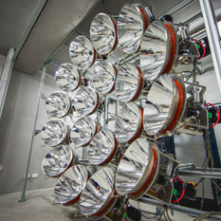
\includegraphics[width=0.5\textwidth]{images/antenna_array}
 \end{center} 
 \caption{Example figure.}
 \label{fig:antenna_array}
\end{figure}


  \chapter{Literature Review}
\vspace{-1.4em}


  \chapter{Methodology}
\vspace{-1.4em}

Note that methodology varies according to project type. Consider the engineering
tools you've learned throughout your degree in ANU to generate your results ---
this may also include the systems engineering approach.

\section{Modelling}
\subsection{Aerodynamic Surfaces}
\subsection{Rotor Forces}
\subsection{Dynamics}

\section{Trajectory Optimisation}
The matlab library OptimTrajectory **intext** was used to solve the optimisation problem for the transition trajectory. OptimTrajectory utilises matlab's fmincon solver.

\subsection{Model Setup}
The aircraft model discussed above was arraged into a statespace representation. 
\[
Y=\begin{bmatrix} x&z&\theta&\dot{x}&\dot{z}&\dot{\theta}\end{bmatrix}^T,
U=\begin{bmatrix} \omega_{f}&\omega_{r}&\epsilon&\delta_{e}\end{bmatrix}^T
\]
\subsection{Constraints}
The constraints for the trajectory optimisation were as follows.
\[
Y_{initial}=\begin{bmatrix}-400 &-50&0**&0&0&0\end{bmatrix}^T
\]
\[
Y_{final}=\begin{bmatrix}0 &-10&0&0&0&0\end{bmatrix}^T
\]
\[
Y_{upper}=\begin{bmatrix} 0&-10&\pi/2&30&\infty&\infty\end{bmatrix}^T
\]

\subsection{Initialisation}
\subsection{Mesh Refinment}
\subsection{Solution}

\section{Control}
\subsection{LQR}
\subsection{Lateral Stabilistaion}
\subsection{Hover}
\subsection{Level Flight}
\subsection{Landing Approach}

\section{Simulation Enviroment}
\subsection{Rotor Model}

\section{Safety Features}
\subsection{Altitude Floor}
The Altitude floor is a minimum altitude that if exceeded with cease the control input overides, returning controll to the stock Ardupilot controller. Fig X *FIGURE OUT FIGURE AND NAMING IN LATEX* show that the stock controllers do not wind up and the aircraft stably returns to the stock trajectory.
\subsection{State Error Disconnect}
another method for rejecting the landing sequence is if the norm of the state error surpasses a preset limit. This triggers in two cases, the first is the aircraft failing to track the trajectory ref figure X, the second being a mismatch in the inital condition for example if the trajectory had not been updated and was made for a different altitude approach.


  \chapter{Results and Analysis}
\vspace{-1.4em}

When presenting your results, it is important that you organise them in an orderly manner to avoid clusters of information. Be critical and properly analyse what the results mean. Provide insightful discussion and explanation. Consider using other published articles to support or argue your results. Make sure it clear which work are yours and which are background materials. Also, include the implication of your results.

\section{Experimental Results}

\section{Subheading 1} 
How to reference Figure ~\ref{table:example}.

\begin{table}[ht]
    \begin{center} 
        \caption{Table captions are above tables. Tables are to be centered on the page.} 
        \begin{tabular}{ccc} 
            \toprule 
            No & Student & Task \\ 
            \midrule 
            1 & A & X \\ 
            2 & B & Y \\ 
            3 & C & Z \\ 
            \bottomrule 
        \end{tabular} 
        \label{table:example} 
    \end{center} 
\end{table}

\section{Analysis and Discussion}

\section{Subheading 2}

\subsection{How to do math equations}
% \( and \) tell latex to do an inline equation. \[ and \] creates a new, separate line for the equation. equation and math environments create a dedicated space for maths equations, with equation numbers that can be referenced.
The well known Pythagorean theorem \(x^2 + y^2 = z^2\) was proved to be invalid for other exponents. Meaning equation \ref{pythag_fail} has no integer solutions:  
\[x^n + y^n = z^n\]

\begin{equation}
    x^n + y^n = z^n
    \label{pythag_fail}
\end{equation}

  \chapter{Conclusions and Future Development}
\vspace{-1.4em}

Provide an answer to your research question or evaluation of overall results given. Discuss what worked well and did not work well in your research. Outline the limitations of approach, methodology, data or research. Give suggestions/recommendations for future work.  
  %\chapter{Further Work}
\vspace{-1.4em}

  %\chapter{Figure and Equations formatting}
\vspace{-1.4em}

\section{cut outs}

\subsection{wireless comms chapter 2}
Another factor which has a strong influence on the fading channel is the Doppler Effect. The Doppler Effect 
occurs when a receiver or transmitter moves location as seen in Figure~\ref{fig:Doppler}. 
\begin{figure}[ht]
 \begin{center}
 %\includegraphics[width=12.5cm]{images/q4a}
%trim option's parameter order: left bottom right top
 \includegraphics[trim = 26.9mm 227mm 66.4mm 26.4mm, clip, width=12.5cm]{images/Doppler}
 \end{center} 
 \vspace{-1cm}
 \caption{Multipath Induced Doppler Effect~\cite{Goldsmith_2005}}
 \label{fig:Doppler}
\end{figure}
The movement of the receiver or transmitter affects the relative locations of reflectors in the wireless 
environment. As stated earlier the reflectors allow alternate paths for signal propagation to the receiver. 
As the relative location of objects change when the receiver or transmitter move, then a different set of 
multipath signals are experienced at the receiver. This phenomenon gives rise to the apparent time-varying 
nature of the channel and leads to rapid changes in the signal strength over small distances.

\subsection{system model chapter 3}
Nakagami-m Fading
The fading amplitude ($H$) in a wireless channel is generally modelled as Nakagami-m distributed (REFERENCE). As m approaches infinity, the Nakagami distribution approaches one and this scenario represents the case of no fading. Setting the value of m to one, results in the well known case of Rayleigh fading and this type of is used ubiquitously throughout this thesis. Thus, it is evident that different values for m result in different fading distributions which are relevant to different transmission environments.





\section{Attenuation in the Wireless Medium}

example code

\textbf{matlab figures}
\begin{figure}[ht]
 \begin{center}
  %\includegraphics[width=12.5cm]{images/q4a}
%trim option's parameter order: left bottom right top
  \includegraphics[trim = 32.5mm 94mm 31mm 94mm, clip, width=12.5cm]{images/q2iii}
  \end{center}

 \vspace{-1cm}
 %\includegraphics[width=12.5cm]{images/propagation_effects}
 \caption{Path loss, shadowing, and multipath versus distance~\cite{Goldsmith_2005}}
 \label{fig:prop_effects}
\end{figure}


Italics
\textit{large-scale propagation effects} 
\hilight{($100$-$1000$ m)}


Subequations
\begin{align}
 y(x) &= \sum_0^{\infty}a_nx^{n+r}     \label{eqn:frobenius 6}\\
 \implies y'(x) &= \sum_0^{\infty}(n+r)a_nx^{n+r - 1}	\label{eqn: frobenius 7}  \\
 \implies y''(x) &= \sum_0^{\infty}(n+r-1)(n+r)a_nx^{n+r - 2}	\label{eqn: frobenius 8} 
\end{align}


matlab code put in here
\begin{verbatim*}
 
\end{verbatim*}


  %=============================================================================
  %      Appendix
  %=============================================================================
  \appendix
  \renewcommand{\chaptermark}[1]{\markboth{Appendix \thechapter\ #1}{}}
  \chapter{Apprendix A: The First}

Manage your references and present them here in order.
  \chapter{Appendix B: The Second}

Manage your references and present them here in order. 
  
  
  %=============================================================================
  %      Bibliography
  %=============================================================================
  \renewcommand{\bibsection}{}
  \chapter*{Bibliography}
  \addcontentsline{toc}{chapter}{Bibliography}
  \bibliographystyle{abbrvnat}
  \bibliography{references_file}


\end{document}
